\documentclass{beamer}
\mode<presentation>
\usetheme[compress]{Berlin}
\usecolortheme{beaver}
\setbeamertemplate{navigation symbols}{}
\setbeamertemplate{footline}{}
\setbeamerfont{footnote}{size=\tiny}
\usepackage{hyperref}
\hypersetup{linkcolor=}
\usepackage[compatibility=false]{caption}
\usepackage{subcaption}
\usepackage{algorithm}
\usepackage{algpseudocode}
\usepackage{IEEEtrantools}
\usepackage{amsmath,amssymb,mathtools,bm,etoolbox}

\title{Photometric Classification \\ with Thompson Sampling}
\subtitle{}
\institute{Supervisors: \\Cheng Soon Ong and Christian Wolf}
\author[Alasdair Tran]{Alasdair Tran \\ \texttt{u4921817}}
\date{\footnotesize{13 Oct 2015}}
\setbeamertemplate{headline}{} % hide header

\newcommand{\A}{\mathpzc{A}}
\newcommand{\X}{\mathcal{X}}
\newcommand{\Y}{\mathcal{Y}}
\newcommand{\Unlabelled}{\mathcal{U}}
\newcommand{\Labelled}{\mathcal{L}}
\newcommand{\R}{\mathcal{R}}
\newcommand*{\argmin}{\operatornamewithlimits{argmin}\limits}
\newcommand*{\argmax}{\operatornamewithlimits{argmax}\limits}

\providecommand\given{}
\DeclarePairedDelimiterXPP\E[1]{\mathbb{E}}{[}{]}{}{
	\renewcommand\given{  \nonscript\:
		\delimsize\vert
		\nonscript\:
		\mathopen{}
		\allowbreak}
	#1
}
\DeclarePairedDelimiterXPP\Prob[1]{\mathbb{P}}{(}{)}{}{
	\renewcommand\given{  \nonscript\:
		\delimsize\vert
		\nonscript\:
		\mathopen{}
		\allowbreak}
	#1
}

\begin{document}
	
\begin{frame}
	\titlepage
\end{frame}

% % % % % % % % % % % % % % % % % % % % % % % % % % % % % % % % % % % % % % % % % % % % % 
\section{Dataset}
\begin{frame}{Sloan Digital Sky Survey}
	Photometric measurements of 800 million objects, out of which
	3 million objects are spectroscopically labelled.
	\begin{figure}
		\centering
		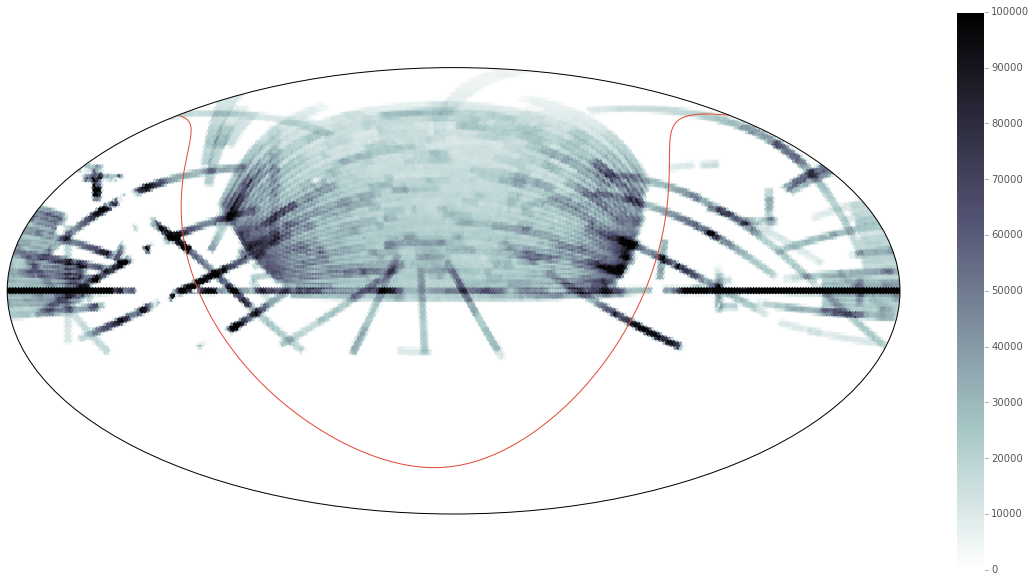
\includegraphics[width=\textwidth]{images/sdss_coverage}
	\end{figure}
\end{frame}



\begin{frame}{Sloan Digital Sky Survey}
	Photometric measurements of 800 million objects, out of which
	3 million objects are spectroscopically labelled.
\begin{figure}[tbp]
	\centering
	\begin{subfigure}{.5\textwidth}
		\centering
		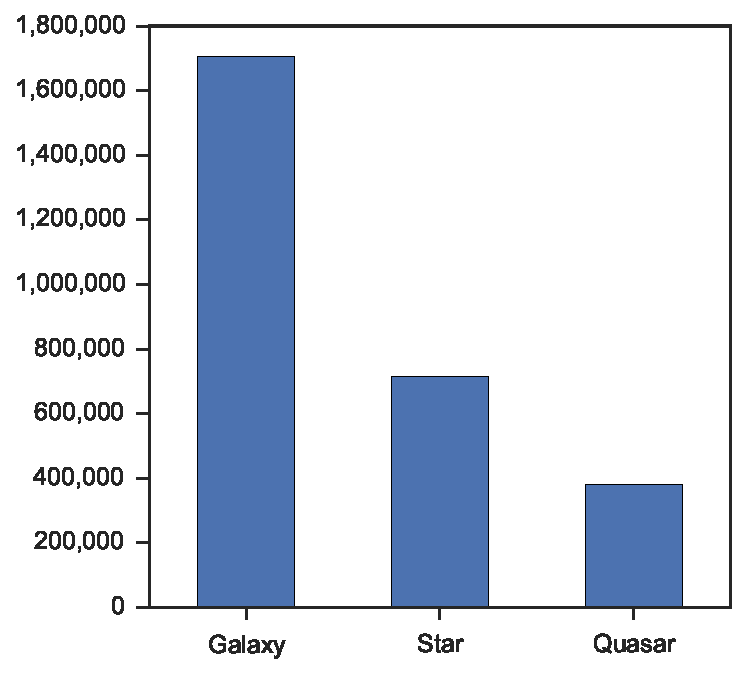
\includegraphics[width=0.99\textwidth]{../thesis/figures/2_astro/sdss_class_distribution}
		\caption{SDSS Dataset}
		\label{fig:class_dist_sdss}
	\end{subfigure}%
	\begin{subfigure}{.5\textwidth}
		\centering
		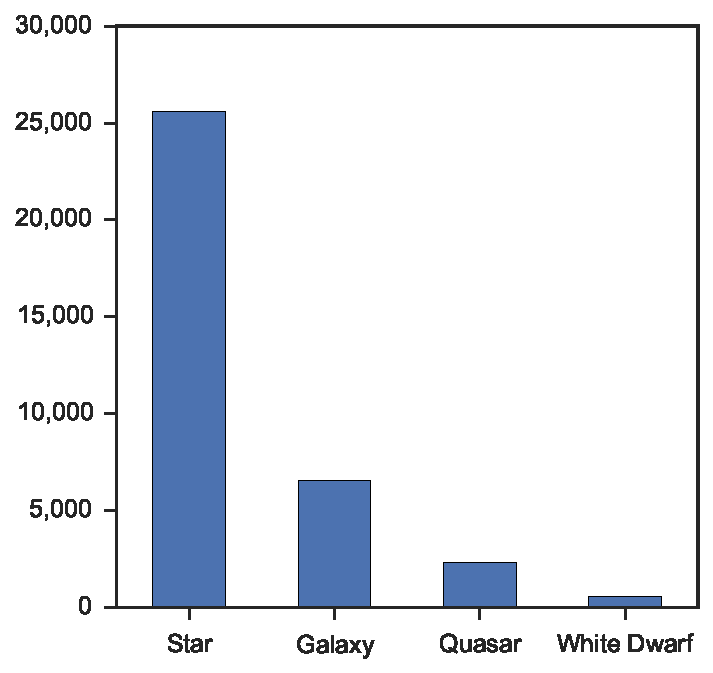
\includegraphics[width=0.99\linewidth]{../thesis/figures/2_astro/vstatlas_class_distribution}
		\caption{VST ATLAS Dataset}
		\label{fig:class_dist_vst}
	\end{subfigure}
	\label{fig:class_dist}
\end{figure}
\end{frame}


\begin{frame}{Photometry vs Spectroscopy}
	\begin{figure}
		\centering
		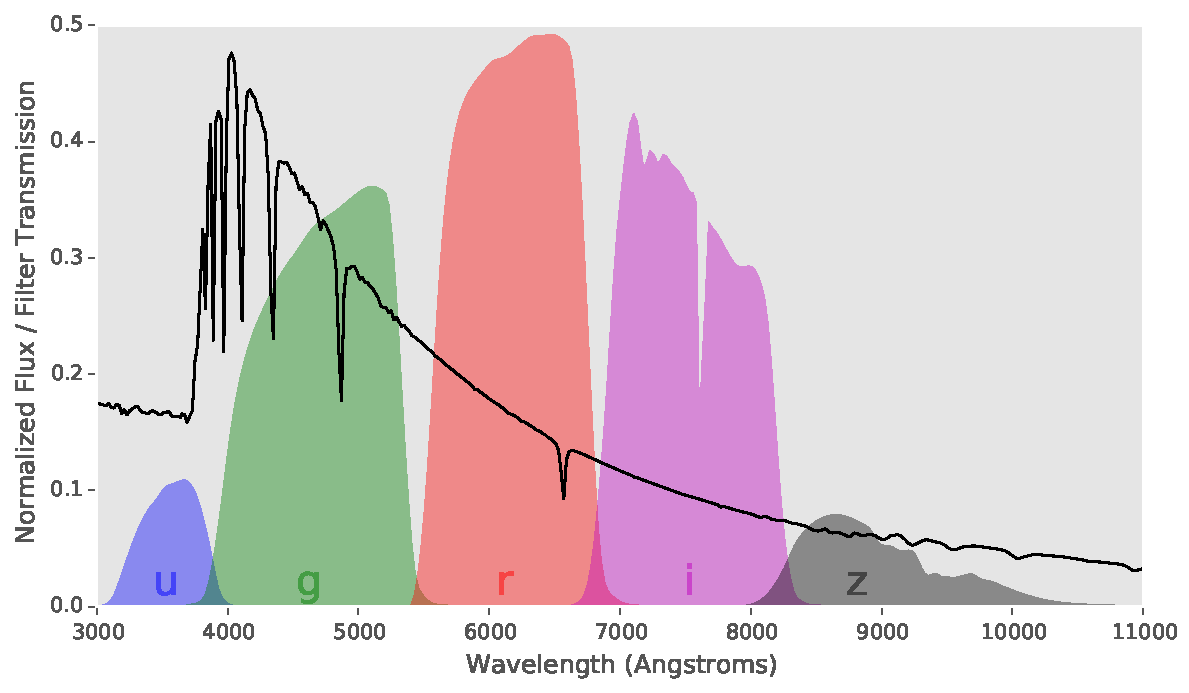
\includegraphics[width=\textwidth]{images/vega}
		\caption{SDSS Filters and Vega Spectrum}
	\end{figure}
\end{frame}

\section{Active Learning}
\begin{frame}{Active Learning Motivation}
	\begin{itemize}
		\item To construct the training set, one solution is to take a random sample objects for labelling.
		\item But labelling is expensive.
		\item Can we be smarter in choosing which objects for labelling?
	\end{itemize}
\end{frame}

\section{Active Learning}
\begin{frame}{Active Learning Algorithm}
	\begin{algorithm}[H]
		\label{alg:active}
		\begin{algorithmic}[1]
			\Procedure {ActiveLearner}{$\Unlabelled$, $\Labelled$, $h$, $r$ $n$, $t$}
			\While {$|\Labelled| < n$}
			\State $E$ $\leftarrow$ random sample of size $t$ from $\Unlabelled$
			\State $\bm{x}_* \leftarrow \argmax_{\bm{x} \in E} r(\bm{x})$
			\State $y_* \leftarrow$ ask the expert to label $\bm{x}_*$
			\State $\Labelled \leftarrow \Labelled  \cup (\bm{x}_*, y_*)$
			\State $\Unlabelled \leftarrow \Unlabelled \setminus \bm{x}_*$
			\State $h_\Labelled(\bm{x}) \leftarrow$ retrain the classifier
			\EndWhile
			\EndProcedure
		\end{algorithmic}
	\end{algorithm}
\end{frame}

\begin{frame}{Active Learning: Uncertainty Sampling Heuristics}
	\begin{itemize}
		\item Pick the example whose prediction vector $p$ displays the greatest Shannon entropy
		(information content):
		\begin{align*}
			r_S(\bm{x}) &= -\sum_{c \in \Y} \Prob{y(\bm{x}) = c} \log \big[\Prob{y(\bm{x}) = c} \big]
		\end{align*}
		\item Pick the example with the smallest margin (difference between
		the two largest values in the prediction vector $p$):
		\begin{align*}
			r_M(\bm{x}) &= \Big|  \Prob{y(\bm{x}) = c^{(1)}} -  \Prob{y(\bm{x}) = c^{(2)}} \Big|
		\end{align*}
	\end{itemize}
\end{frame}


\begin{frame}{Active Learning: Query by Bagging Heuristics}
	\begin{enumerate}
		\item Use bagging to train $B$ classifiers $f_1, f_2, ..., f_B$.
		\item Rank candidates by disagreement among $f_i$:
		\begin{itemize}
			\item Margin-based disagreement: average the prediction of $f_i$ and choose the
			example with the smallest margin.
			\item Choose the example with the highest average Kullback-Leibler divergence
			from the average:
			\begin{align*}
				r_{QBB,KL}(\bm{x}) = \dfrac{1}{B} \sum_{b=1}^B D_{\mathrm{KL}}(P_b\|Q)
			\end{align*}
		\end{itemize}	
	\end{enumerate}
\end{frame}

\begin{frame}{Active Learning: Loss Function Heuristic}
	\begin{itemize}
		\item Expected squared loss can be decomposed into three terms:
		\begin{IEEEeqnarray*}{lCl}
			\E{\text{Squared Loss}} &=& \text{Bias}^2 + \text{Variance} + \text{Noise}
		\end{IEEEeqnarray*}
		\item Pick the example that will cause the greatest drop in variance of the unlabelled pool:
			\begin{IEEEeqnarray*}{lCl}
				r_V(\bm{x}) &=& \sum_i^k \Prob{y(\bm{x}) = i} V_{\Labelled \cup \bm{x}}
			\end{IEEEeqnarray*}
	\end{itemize}
\end{frame}

\begin{frame}{Active Learning: Classifier Certainty Heuristic}
	\begin{itemize}
		\item The entropy of the classifier's predictions on $\Unlabelled$ is
		\begin{IEEEeqnarray*}{lCl}
			CC_{\Labelled} &=& - \sum_{\bm{u} \in \Unlabelled} \sum_{c \in \Y} \Prob{y(\bm{u}) = c} \log \big[\Prob{y(\bm{u}) = c} \big]
		\end{IEEEeqnarray*}
		\item Pick the example that is expected to increase the classifier's
		prediction certainty by the the greatest amount:
		\begin{IEEEeqnarray*}{lCl}
			r_{CC}(\bm{x}) &=& -\sum_{c\in \Y} \Prob{y(\bm{x}) = c} CC_{\Labelled \cup \bm{x}}
		\end{IEEEeqnarray*}
	\end{itemize}
\end{frame}


\begin{frame}{Multi-arm bandit Problem}
	\begin{itemize}
		\item A gambler stands in front a slot machine with $n$ levers.
		\item Each lever emits a reward of unknown distribution.
		\item Goal: maximise lifetime rewards
	\end{itemize}
\end{frame}

\algblockdefx[Forall]{Foreach}{Endforeach}%
[1]{\textbf{for each} #1 \textbf{do}}%
{\textbf{end for}}

\begin{frame}{Thompson Sampling}
\begin{algorithm}[H]
	\caption{Thompson sapmling}
	\label{alg:thompson}
	\begin{algorithmic}[1]
		\Procedure {ThompsonSampling}{$\R$, $\bm{\mu}$, $\bm{\sigma}$, $\bm{\tau}$}
		\Foreach {$t \in \{1, 2, ..., n\}$}
		\Foreach {$r \in \R$}
		\State $\bm{\nu}_r' \leftarrow$ draw a sample from $N(\bm{\mu_r}, \bm{\sigma_r})$
		\Endforeach
		\State $r_* \leftarrow \argmax_{r \in \R}\bm{\nu}_r'$
		\State Observe reward $w_{*}$
		\State Update $\bm{\mu}_{*}$
		\State Update $\bm{\sigma}_{*}$
		\Endforeach
		\EndProcedure
	\end{algorithmic}
\end{algorithm}
\end{frame}



\begin{frame}{Learning Curves with Random Sampling}
\begin{figure}[tbp]
	\centering
	\begin{subfigure}{.5\textwidth}
		\centering
		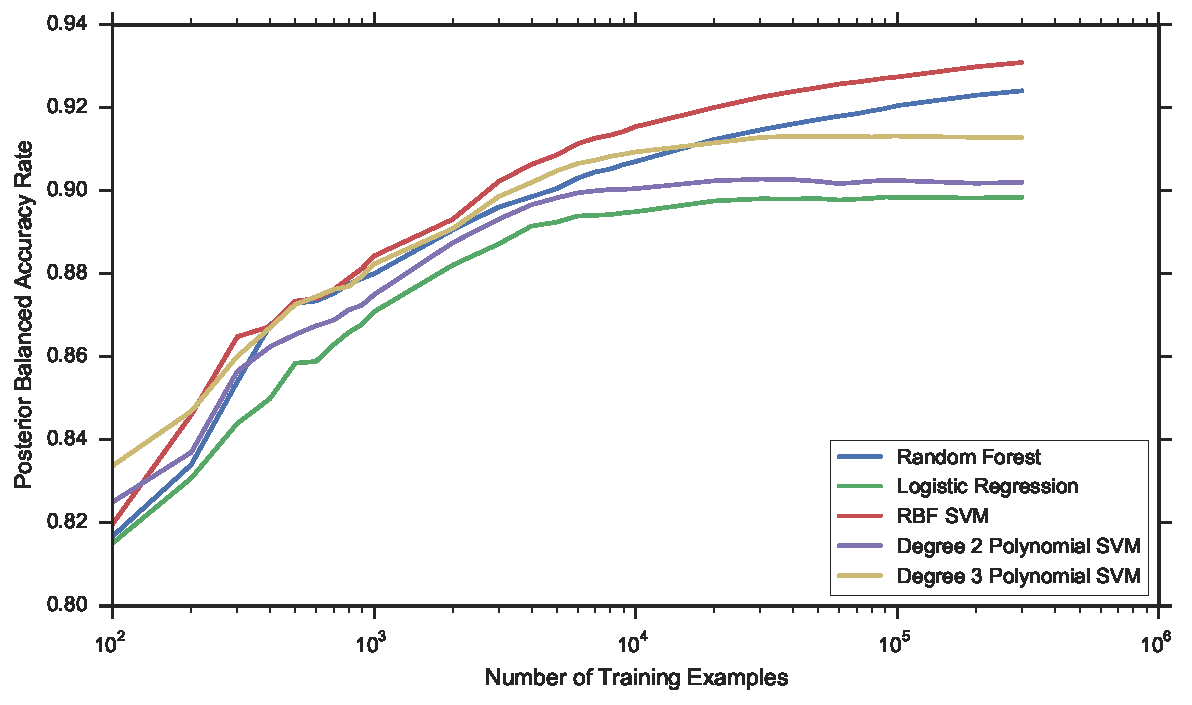
\includegraphics[width=0.99\textwidth]{../thesis/figures/4_expt1/sdss_learning_curves}
		\caption{With SDSS data}
		\label{fig:sdss_learning_curves}
	\end{subfigure}%
	\begin{subfigure}{.5\textwidth}
		\centering
		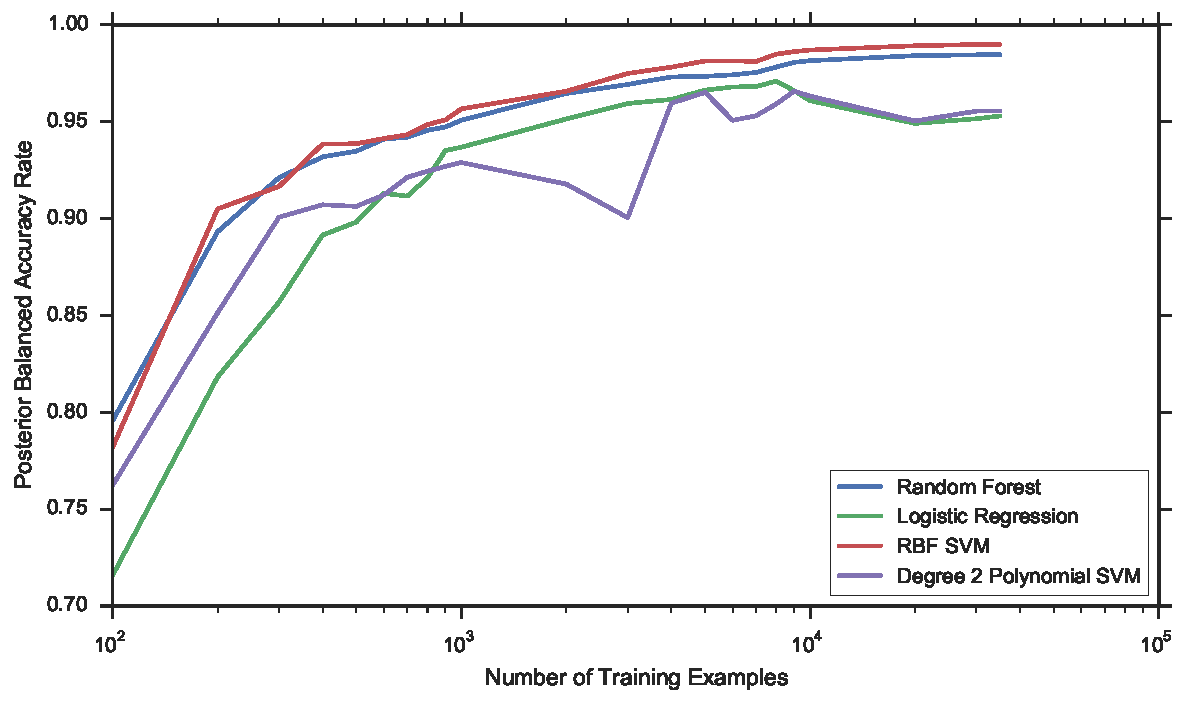
\includegraphics[width=0.99\linewidth]{../thesis/figures/4_expt1/vstatlas_learning_curves}
		\caption{With VST ATLAS data}
		\label{fig:vstatlas_learning_curves}
	\end{subfigure}
	\label{fig:learning_curves}
\end{figure}
\end{frame}




\begin{frame}{Learning Curves with Acive Learning}
	Balanced Pool with Logistic Regresion
	\begin{figure}[tbp]
		\centering
		\begin{subfigure}{.5\textwidth}
			\centering
			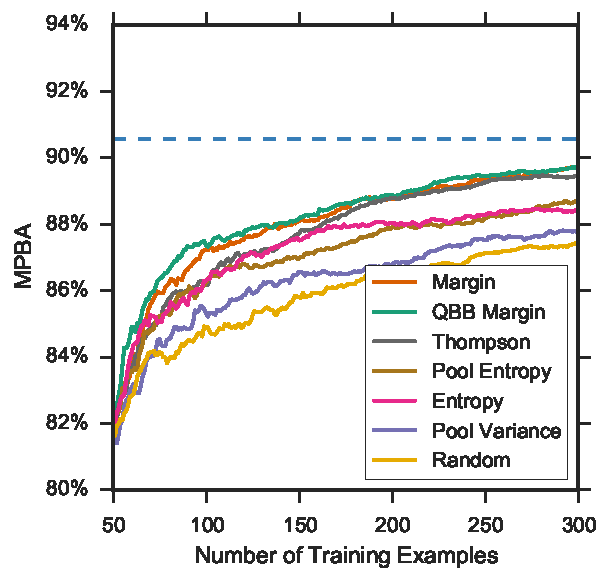
\includegraphics[width=0.99\textwidth]{../thesis/figures/5_active/sdss_bl_ind_upper}
			\caption{SDSS Dataset}
		\end{subfigure}%
		\begin{subfigure}{.5\textwidth}
			\centering
			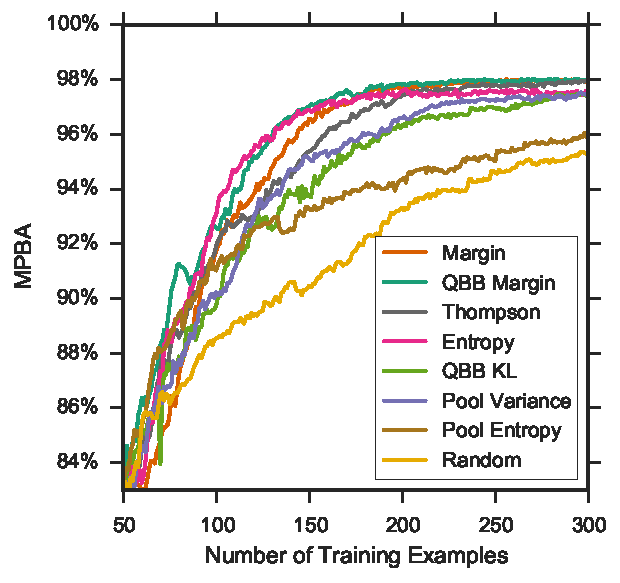
\includegraphics[width=0.99\linewidth]{../thesis/figures/5_active/vstatlas_bl_ind_upper}
			\caption{VST ATLAS Dataset}
		\end{subfigure}
	\end{figure}
\end{frame}

\begin{frame}{Learning Curves with Active Learning}
	Unbalanced Pool with Logistic Regresion
	\begin{figure}[tbp]
		\centering
		\begin{subfigure}{.5\textwidth}
			\centering
			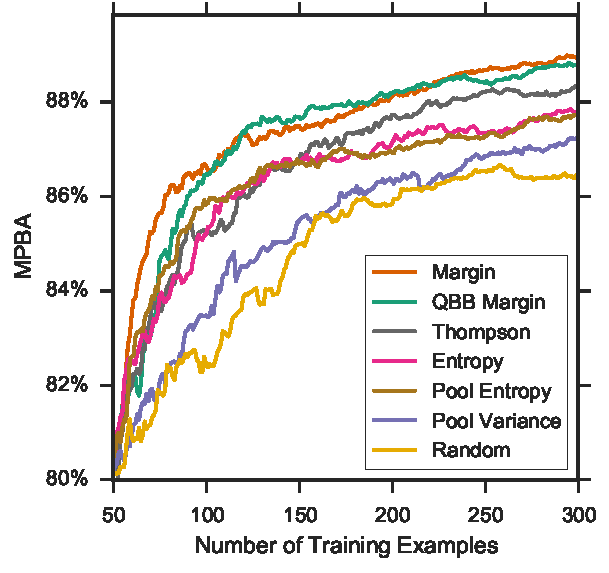
\includegraphics[width=0.99\textwidth]{../thesis/figures/5_active/sdss_ul_ind_upper}
			\caption{SDSS Dataset}
		\end{subfigure}%
		\begin{subfigure}{.5\textwidth}
			\centering
			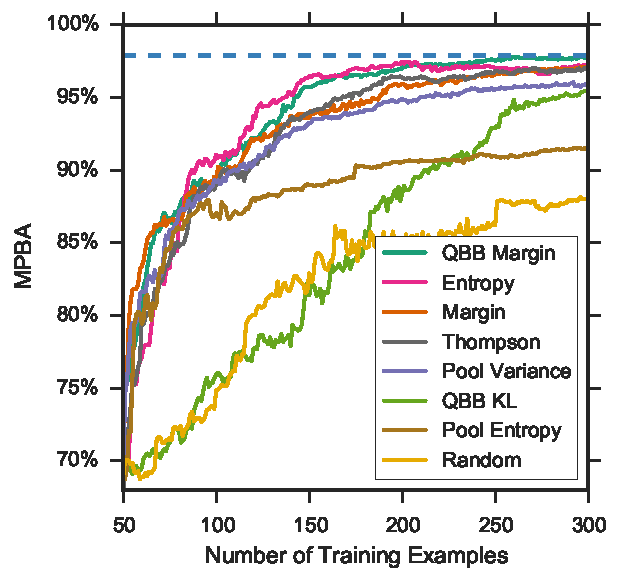
\includegraphics[width=0.99\linewidth]{../thesis/figures/5_active/vstatlas_ul_ind_upper}
			\caption{VST ATLAS Dataset}
		\end{subfigure}
	\end{figure}
\end{frame}

\begin{frame}{Heuristic Selection}
	VST ATLAS, Unbalanced, Logistic Regression.
		\begin{figure}[tbp]
			\centering
			\begin{subfigure}{.5\textwidth}
				\centering
				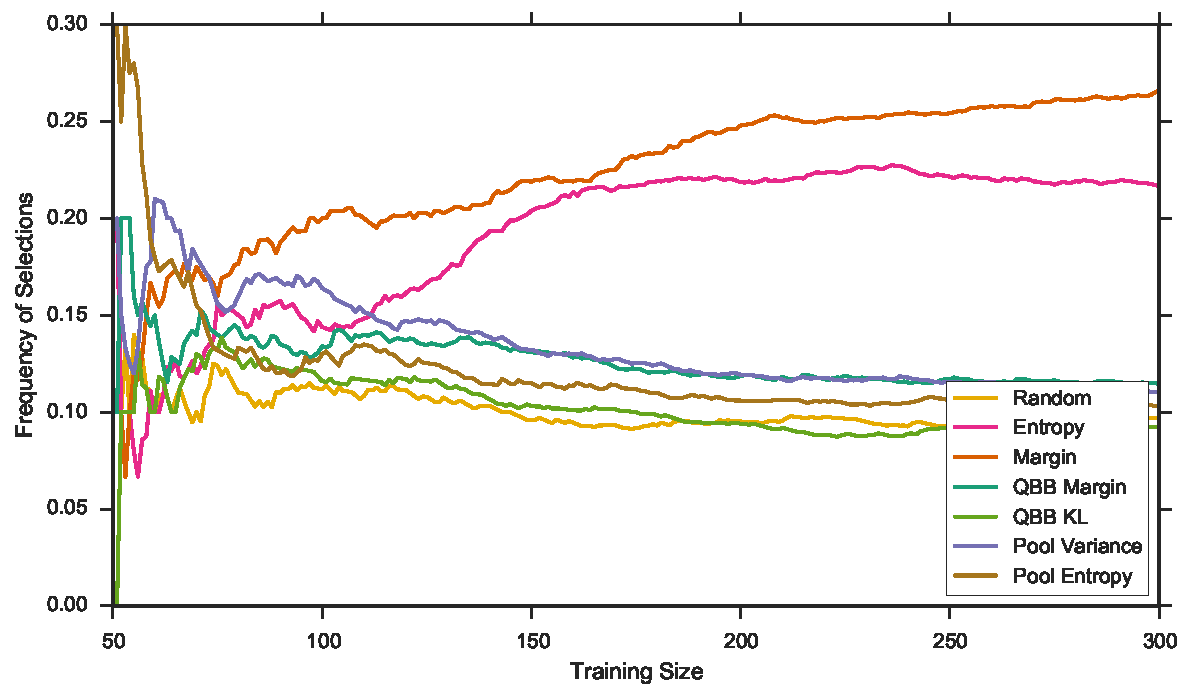
\includegraphics[width=0.99\textwidth]{../thesis/figures/5_thompson/vstatlas_ul_frequencies}
				\caption{Frequency}
			\end{subfigure}%
			\begin{subfigure}{.5\textwidth}
				\centering
				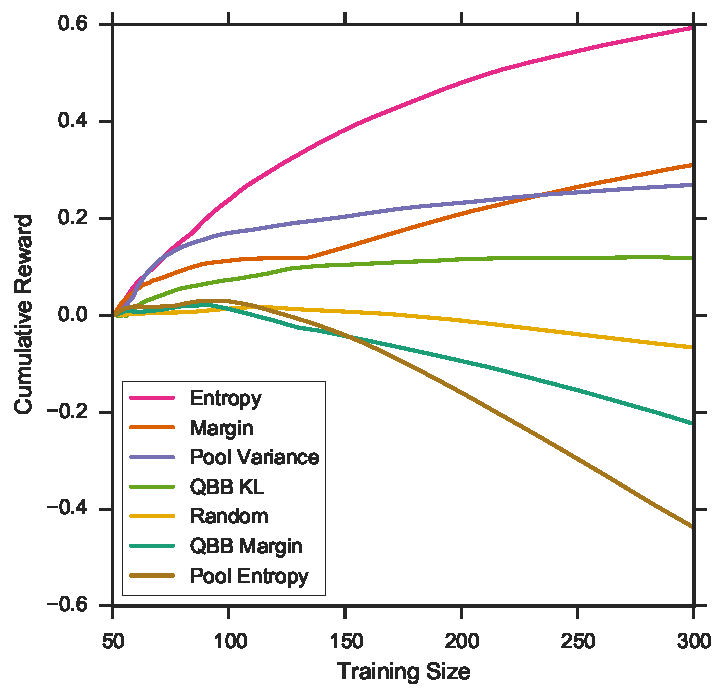
\includegraphics[width=0.99\linewidth]{../thesis/figures/5_thompson/vstatlas_ul_sum_rewards}
				\caption{Cumulative Rewards}
			\end{subfigure}
		\end{figure}
\end{frame}

\begin{frame}{Drifting Rewards}
	VST ATLAS, Unbalanced, Logistic Regression.
	\begin{figure}[tbp]
		\centering
		\begin{subfigure}{.5\textwidth}
			\centering
			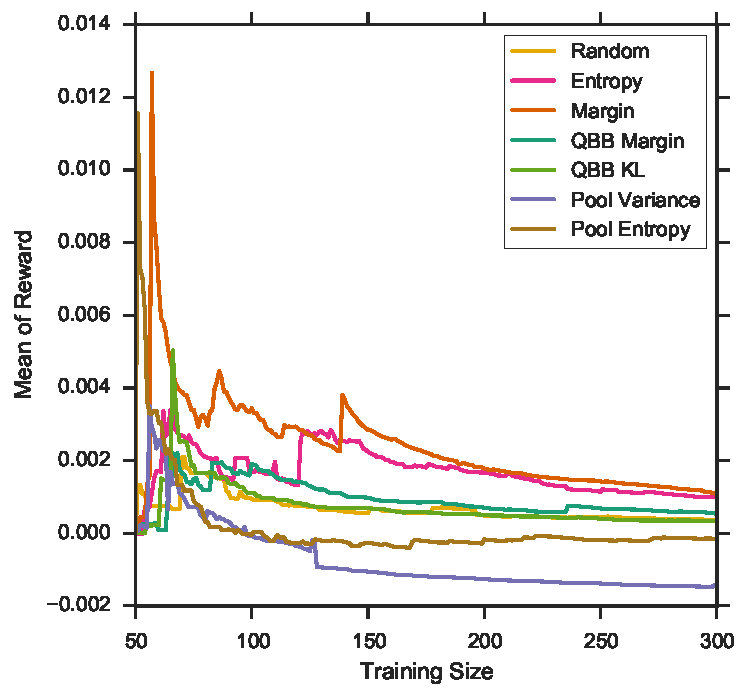
\includegraphics[width=0.99\textwidth]{../thesis/figures/5_thompson/vstatlas_ul_avg_rewards}
			\caption{Frequency}
		\end{subfigure}%
		\begin{subfigure}{.5\textwidth}
			\centering
			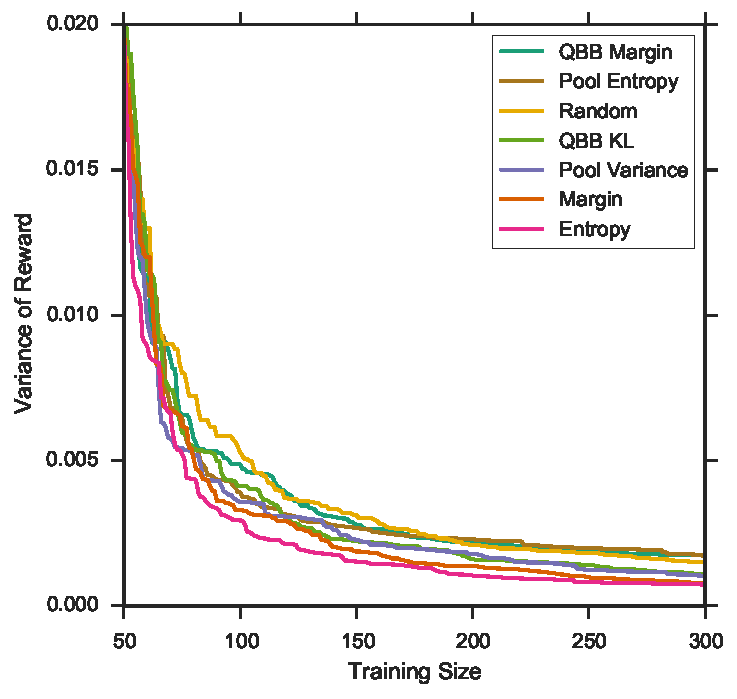
\includegraphics[width=0.99\linewidth]{../thesis/figures/5_thompson/vstatlas_ul_sigmas}
			\caption{Cumulative Rewards}
		\end{subfigure}
	\end{figure}
\end{frame}








\begin{frame}{Concluding Remarks}
	\begin{itemize}
		\item Dynamic Thompson Sampling approach to address	the reward drifting problem
		\item Theoretical analysis of convergence.
		\item Batch active learning.
	\end{itemize}
\end{frame}


\end{document}
